%!TEX encoding = UTF-8 Unicode
% -*- coding: UTF-8; -*-
% vim: set fenc-utf-8

\chapter{Diagrammes de classe de conception}
\label{s:classe_conception}

Ce chapitre présente les différents diagrammes de classe de conception de \textit{VisualLigue}.

\section{Couche présentation}
\label{sec:couche_presentation}

La figure \ref{fig:vue_classes_conception_diag} présente le diagramme de classe de la couche présentation(vue).
La technologie JavaFX est utilisée en union avec le constructeur d'interface graphique \textit{Scene Builder}.
Il y a donc un fichier FXML associé à chacune de ces classes qui contient le code des éléments graphiques.
De prime abord, la classe \textit{RootLayoutController} représente la fenêtre de base de l'application.
Celle-ci contient la barre de menu principal, qui permet d'exécuter la majorité des fonctionnalités du logiciel.
C'est pour cela que ce contrôleur contient une majorité des méthodes permettant la gestion des événements.
Par ailleurs, le patron de conception \textit{Observateur} est utilisé afin de rediriger la gestion de certains événements vers le \textit{RootLayoutController}.
Cela permet d'éviter une duplication du code de gestion des événements tout en maintenant le couplage bas.
Ainsi, la même fonctionnalité peut être exécutée par la barre de menu ou par un bouton dans un autre contrôleur.


%\begin{figure}[htpb]
    %\centering
    %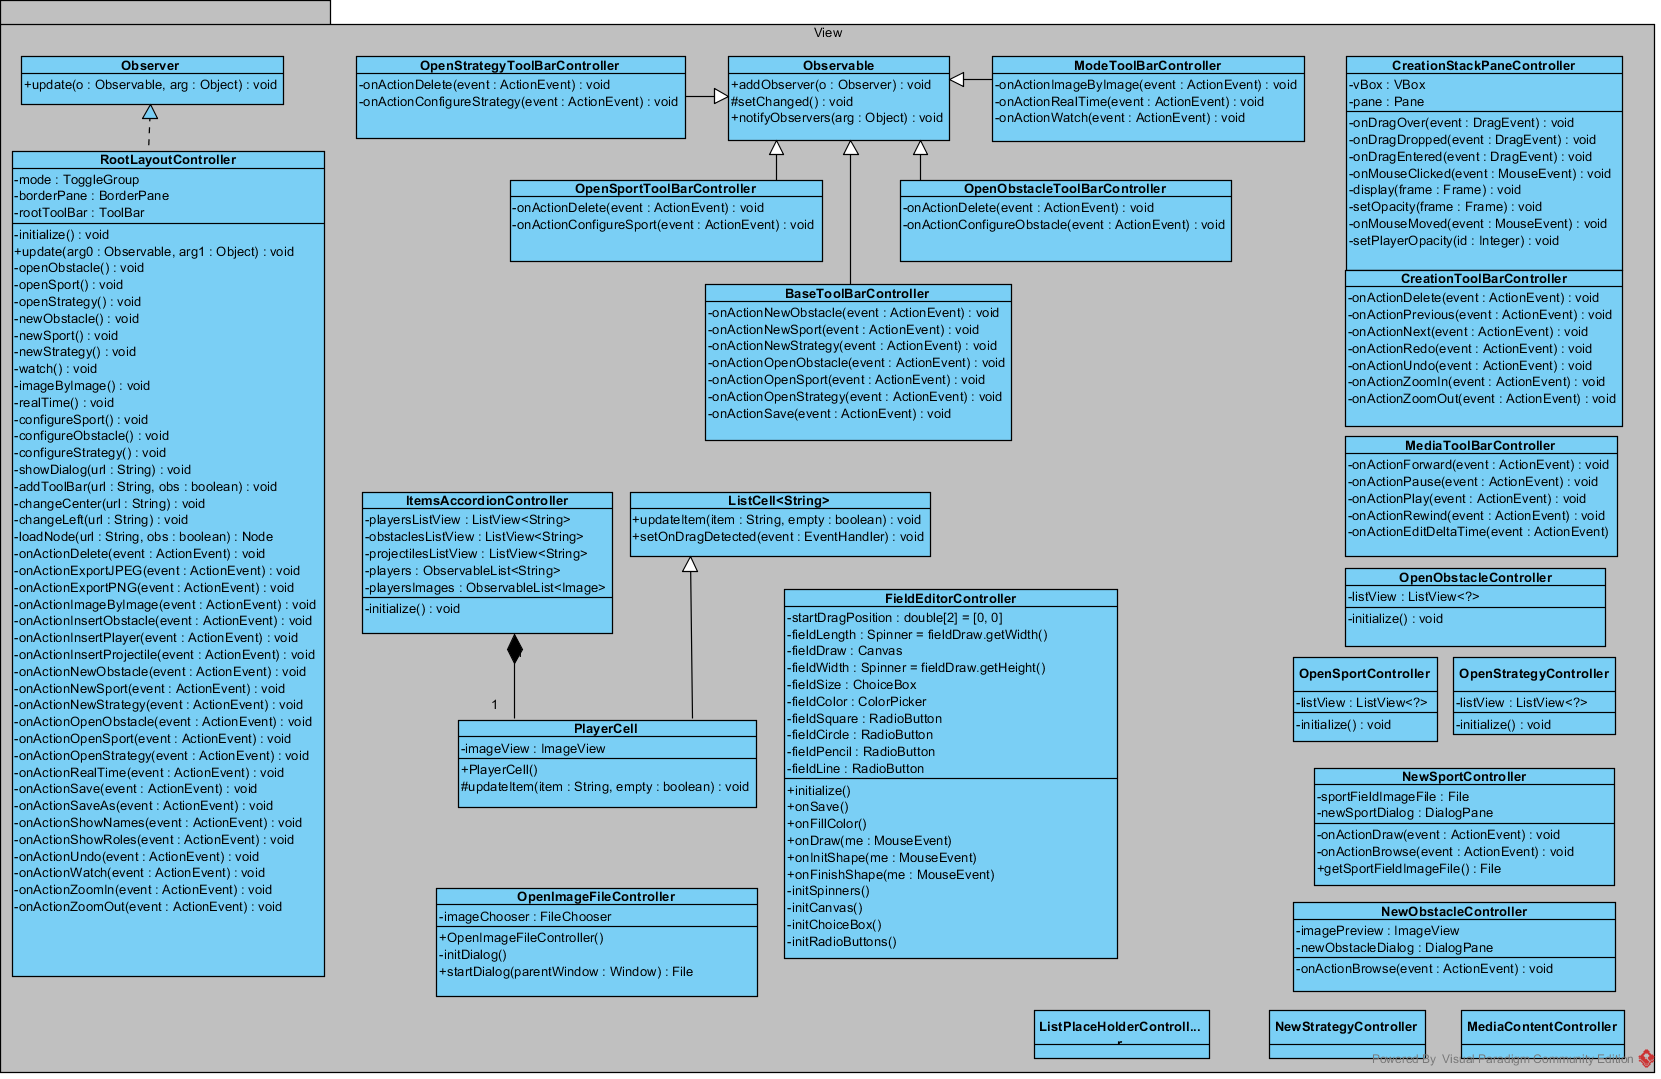
\includegraphics[scale=0.6]{fig/vue_classes_conception_diag.png}
    %\caption{Diagramme de classes de conception de la couche présentation}
    %\label{fig:vue_classes_conception_diag}
%\end{figure}